\documentclass[12pt]{article}
\usepackage{float}
\usepackage{graphicx}
\usepackage{amsmath}
\usepackage{tikz}
\usepackage{pgfplots}
\usepackage[
backend=biber,
style=numeric,
sorting=ynt
]{biblatex}
\usepackage[letterpaper,margin=1in]{geometry}
\usepackage{minted}
% \renewcommand{\footnotesize}{\small\spaceskip4pt plus1.5pt}

\pagenumbering{gobble}		
\tolerance9000

\addbibresource{report.bib}
\nocite{*}

\title{Parallelizing Convex Hull}
\author{Claudia Cortell (ccc2223), Kyle Edwards (kje2115), and Avighna Suresh (as6469)}

\begin{document}

  \maketitle
  \newpage

  % \centerline{\bf Parallel Convex Hull Project Proposal}
  \setcounter{section}{0}

  \section{Introduction}

    \begin{figure}[h]
      \centering
      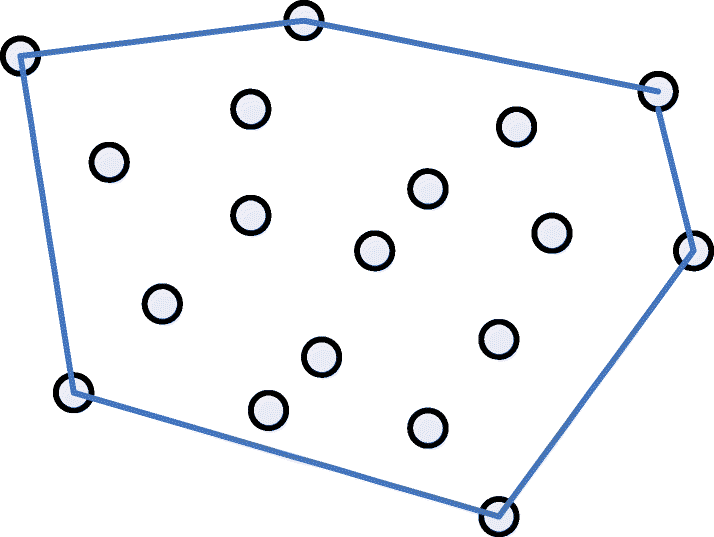
\includegraphics[width=0.6\textwidth]{convex_hull.png}
      \caption{An example of a 2D convex hull.}
    \end{figure}

    \noindent
    Given a set $P$ of $n$ points in a plane, the convex hull of $P$ is the smallest convex polygon containing the points and the largest convex polygon whose vertices are points in $P$.

    \begin{figure}[h]
      \centering
      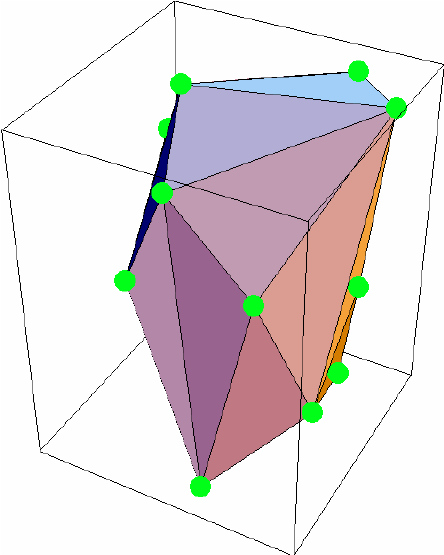
\includegraphics[width=0.3\textwidth]{convex_hull_3d.png}
      \caption{An example of a 3D convex hull.}
    \end{figure}

    Convex hulls also naturally extend to three dimensions. Analogous to how a 2D convex hull is the smallest convex polygon enclosing a set of all points in a plane, a 3D convex hull is the smallest convex polyhedron that completely encloses a set of points in three-dimensional space. The hull itself is made up of flat triangular faces that connect to form the surface of the polyhedron. Every point in the original set either lies on the surface of this polyhedron or inside it, and any line segment connecting any two points within the hull lies completely inside the hull.

    Due to the large number of use cases for convex hulls and the relative lack of already existing parallel algorithms for the problem, our project aims to parallelize an existing convex hull algorithm. Specifically, we aim to implement both sequential and parallel convex hull algorithms in order to compare the increase in speed that parallelization would provide.
  \section{Algorithms} 

  \subsection*{Graham Scan}

    The Graham Scan algorithm provides a simple yet effective approach to computing convex hulls with consistent runtime behavior. The algorithm executes in two main phases: sorting points based on their polar angles, and constructing the hull through point traversal. In the sorting phase, using the point with the lowest y-coordinate as a reference point, the algorithm computes angles between this point, the x-axis, and each remaining point. These angles determine the counterclockwise ordering of points. The hull construction phase uses a stack-based approach to identify hull points: for each point in the sorted sequence, the algorithm removes points from the stack until three consecutive points (the current point and top two stack points) form a counterclockwise turn, then pushes the current point onto the stack. The stack's remaining points form the convex hull once all points have been processed.

    The algorithm runs in $O(n\log n)$ time, as its time complexity is dominated by the initial sorting phase.

  \subsection*{QuickHull (2D)}

  \begin{figure}[h]
    \centering
    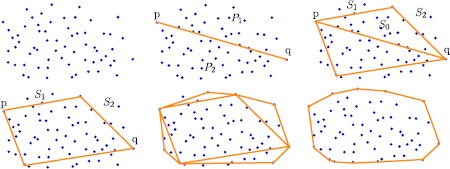
\includegraphics[width=0.8\textwidth]{quick_hull_2d.png}
    \caption{A visual demonstration of the steps of QuickHull.}
  \end{figure}

    \noindent
    The 2D QuickHull algorithm implements a divide-and-conquer approach to constructing convex hulls in 2D space. For point sets of size four or larger (as smaller sets are their own convex hulls by default), the algorithm begins by identifying the points with minimum and maximum $x$-coordinates, which are guaranteed to be part of the final hull. These points create a line that partitions the remaining points into two sets - those above and below the line.

    The core recursive operation processes points relative to a line segment defined by two points. For each recursive call, the algorithm computes cross products to determine which points lie to the left of the oriented line. If fewer than two points remain on the left side, the algorithm returns the first endpoint concatenated with these points. Otherwise, it identifies the point that forms the largest area triangle with the current line segment and recursively processes two new subproblems: points left of the line from the first endpoint to this maximum point, and points left of the line from this maximum point to the second endpoint.

    The algorithm combines the results of processing points above and below the initial line (from leftmost to rightmost point) to form the complete convex hull and is made more efficient by eliminating points that lie inside triangles formed during the recursive process. While the average-case time complexity is $O(n\log n)$, it can degrade to $O(n^2)$ when many points lie on or near the hull.

  \subsection*{QuickHull (3D)}

    The 3D QuickHull algorithm extends 2D QuickHull’s divide-and-conquer approach to constructing convex hulls in 3D space. Unlike 2D QuickHull, which works with lines and points on either side, the 3D version works with triangular faces and points that lie above or below them.

    The algorithm begins with an initialization phase that establishes a foundational tetrahedron with four extreme non-coplanar points that will form the initial structure of the hull. Once the initial tetrahedron is established, the algorithm creates four triangular faces, each represented by three vertices. For each face, the algorithm determines its "outside set" - the collection of remaining points that lie above the face. Similar to 2D QuickHull, determining which side a point lies on relative to a face is done using a cross product, in this case with the vertex normal of the face. The main processing phase recursively refines the hull: for each face that has points in its outside set, find the furthest point and use it to create new faces to create what can be visualized as a cone – the furthest point is connected to each edge of the original face, forming three new triangular faces. Each of these new faces then inherits a subset of points from the original face's outside set, specifically those points that lie above it. The recursive process continues until all faces have empty outside sets, meaning no remaining points lie outside the current hull structure. The final hull is then constructed by collecting all the unique vertices from the faces that survived the refinement process.

    While the worst-case time complexity remains $O(n^2)$ like in 2D, the algorithm often performs much better in practice due to the efficient pruning of points and the fact that most points are typically eliminated early in the process. Furthermore, the branching factor for 3D QuickHull’s recursion is 3 rather than 2.

  \newpage 
  \subsection*{Chan's Algorithm}

    \begin{figure}[h!]
      \centering
      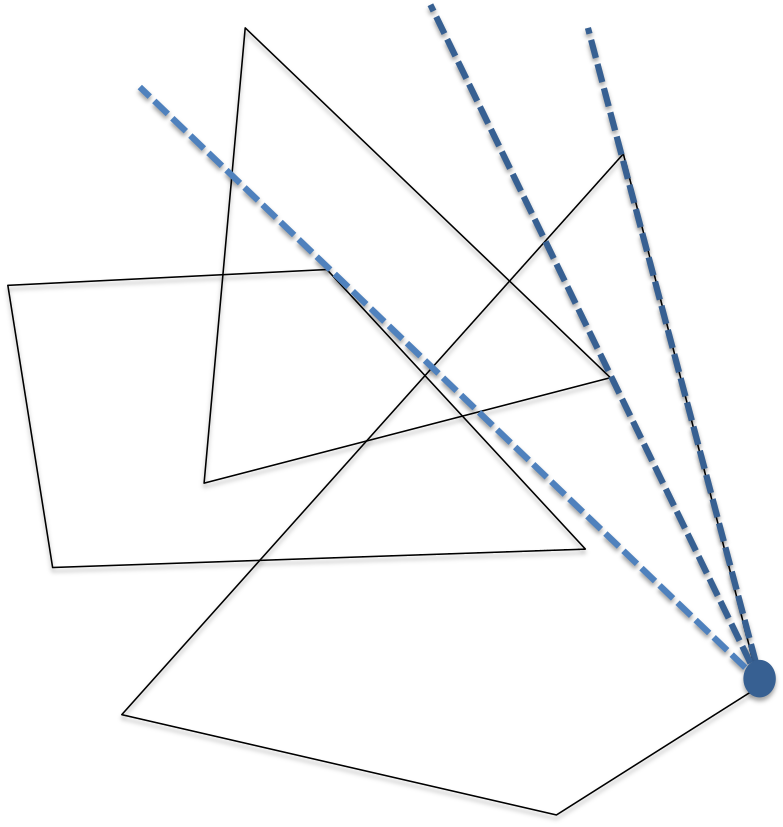
\includegraphics[width=0.6\textwidth]{chans.png}
      \caption{A visual example of Chan's algorithm. More specifically, a visual example of what finding the rightmost point of each sub-hull would look like.}
    \end{figure}
    
    \noindent
    Chan’s algorithm is similar to QuickHull in that it employs a divide-and-conquer approach. Points are first partitioned into K subsets, each subset containing m points. Then, the convex hull of each subset is found using any $O(n\log n)$ convex hull algorithm, each sub-hull’s points being ordered in a counter-clockwise order (in our case, we used QuickHull). Finally, the convex hulls of each subset are merged into the final convex hull using a modified version of another convex hull algorithm known as the gift-wrapping algorithm: starting from a point known to be on the convex hull (e.g. any extreme point), iterate through each point to find the point oriented the most to the right, add that point to the hull, move to that point, and repeat until the initial point is reached. The trick that Chan’s algorithm employs relies on the fact that each sub-hull’s points are ordered, meaning that finding the rightmost point of a sub-hull can be done using a binary search.

    Altogether, finding the convex hull of each sub-grouping of points takes $O(n\log m)$ time, and merging the sub-hulls takes $O(Kh\log m)$ time. Assuming that $m \approx h$, this results in a total time complexity of $O(n\log h)$, making it theoretically the best of the three algorithms.

  \section{Parallelization}
  
    We decided to parallelize the divide-and-conquer algorithms by creating a new spark for each recursive subproblem. In particular, each spark was evaluated using \mintinline{haskell}{rdeepseq} to reduce the number of thunks, as due to the divide-and-conquer nature of each algorithm, points discarded during each recursive subproblem are never used again, meaning it makes sense to determine as soon as possible through reduction to normal form when a point can be discarded in order to save memory. We did not parallelize Graham scan, as our intention was to use it as a benchmark due to its simplicity.

    QuickHull's 2D implementation achieves parallelization by dividing the initial problem into four distinct regions based on extremal points, creating a list of four line segments that form a rough boundary of the point set, and processing each of the four recursive sub-problems in parallel using \mintinline{haskell}{parList}:

    \begin{minted}{haskell}

let topLeft = (minXPoint, maxYPoint)
    topRight = (maxYPoint, maxXPoint)
    bottomRight = (maxXPoint, minYPoint)
    bottomLeft = (minYPoint, minXPoint)
 in
    concat (map (_quickHull2Par 1 points) \
      [topLeft, topRight, bottomRight, bottomLeft] \
      `using` parList rdeepseq)

    \end{minted}

    For each subsequent recursive sub-problem, we also use \mintinline{haskell}{parList} in order to evaluate the two new recursive sub-problems, returning a concatenation of their results.

\begin{minted}{haskell}
concat (map (_quickHull2Par (d + 1) onLeft) nextLines \
  `using` parList rdeepseq)
\end{minted}

  The 3D implementation applies the same parallelization method, focusing instead on a tetrahedron's faces as the primary units of parallel computation. After constructing the initial tetrahedron, the algorithm processes each face independently in parallel:

\begin{minted}{haskell}
concat (map (processPointsParallel 0 epsilon points) initialFaces \
  `using` parList rdeepseq)
\end{minted}

	For Chan’s algorithm, we employed parallelization for finding the convex hulls of each sub-grouping of points. We also turn the resulting list into a vector.

\begin{minted}{haskell}
map (V.force . V.fromList . quickHull2) subPoints \
  `using` parBuffer 32 rdeepseq
\end{minted}

  We also decided to use \mintinline{haskell}{parBuffer} over \mintinline{haskell}{parList}, as the list of sub-groupings is quite large. This greatly reduced the memory footprint, reducing the amount of space used from $\sim$1.5GB to only $\sim$50MB, which thus resulted in better performance. The value 32 was found empirically.

  \section{Design Decisions}

    For generating points, we decided to use a random number generator at runtime rather than a predetermined list of points read from a file. This was done after we observed that the latter approach caused our program to be mostly I/O-bound. Furthermore, random generation of points was not very time consuming. In practice it would probably make more sense to read points from a file, but in our case we wanted to eliminate as many external factors as possible from the total time of the program.

    Instead of finding the number of input points at runtime, we decided to instead pass it in as an argument. For Chan’s algorithm in particular, in order to optimally subdivide the points into sub-groups, the length of the list has to be known. However, when we used \mintinline{haskell}{length ps} to find this value, we found on Threadscope that almost half of the time was spent iterating over the list of points just to calculate the length. As such, we decided to just pass it in as an argument to the function, as we figured that the list passed in would almost always be of finite length anyways.

    For QuickHull, in order to prevent too many sparks from being created, we add a depth limit, controlled by a \mintinline{haskell}{maxDepth} parameter. After experimenting with various depth limits, we did not see a drastic difference in performance, so we picked a depth limit of 100 for 2D and 50 for 3D. It's likely that removing the depth limit altogether would not result in any noticeable decrease in speed.

    For Chan’s algorithm, rather than using the squaring method we spoke of in our proposal to find a suitable value for $m$, we decided to instead calculate it simply as a function of $n$, the number of input points. In particular, using the approximation that $m \approx h$, we deduced that a good approximation was $m\approx3\sqrt n$. This approximation was used due to the fact that, for a circle of area $A$, the circumference with respect to $A$ is equal to $2\sqrt A$, and for a square also of area $A$, the perimeter with respect to $A$ is equal to $4\sqrt A$, thus suggesting that a good general guess for the perimeter of a polygon (analogous to $h$, which itself should approximate $m$) given its area (analogous the the number of points) would be $3\sqrt A$. We also empirically found that this value performed the best by comparing runtimes.

    We started out by creating our own \mintinline{haskell}{Point} class before quickly realizing that we could use the \mintinline{haskell}{Linear} package's \mintinline{haskell}{V2} and \mintinline{haskell}{V3} instead. This helped to reduce the amount of boilerplate code we needed to create.

    For the binary search for Chan’s algorithm, we used the vector library in order to have lists that could be accessed at constant time. When combined with our choice of using rdeepseq, this meant that each vector was immediately ready to be used.

    Finally, we found that increasing the size of the nursery to ~64MB drastically reduced the time spent doing garbage collection. This was especially the case with Chan’s algorithm, where performance nearly doubled. For those wishing to run our code, we suggest increasing the nursery size.

    Some routes that went down that were not successful included using REPA and forcing point evaluation before passing it to the algorithm. In QuickHull, we tried to use REPA to parallelize the calculation of the distance from each point to the line to speed up finding the farthest point from the line. However, there were little performance benefits, since it required converting to and from regular Haskell lists to use parallel strategies. Parallelizing calculating the distances of each point using functions such as parList and parBuffer also did not provide adequate results, as the number of points was very large, and the distance calculation was simple enough that the overhead of creating sparks often outweighed any performance benefits.

  \section{Findings \& Results}

    For all graphs, blue will represent QuickHull in 2D, green will represent Chan's algorithm, and orange will represent QuickHull in 3D. Squares represent linear algorithms, and triangles represent parallel algorithms.

    \begin{figure}[h]
      \centering
      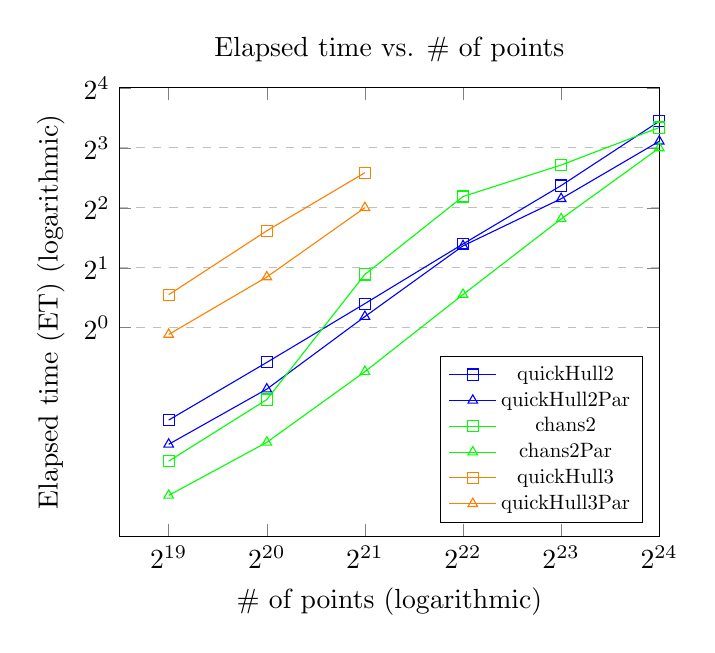
\begin{tikzpicture}
      \begin{axis}[
          title={Elapsed time vs. \# of points},
          xlabel={\# of points (logarithmic)},
          ylabel={Elapsed time (ET) (logarithmic)},
          log basis x = 2,
          log basis y = 2,
          xmode=log,
          ymode=log,
          xmax=16777216,
          ymax=16,
          xtick={524288,1048576,2097152,4194304,8388608,16777216},
          xticklabels={$2^{19}$,$2^{20}$,$2^{21}$,$2^{22}$,$2^{23}$,$2^{24}$},
          ytick={1,2,4,8,16},
          yticklabels={$2^0$,$2^1$,$2^2$,$2^3$,$2^4$},
          legend style={nodes={scale=0.75, transform shape}},
          legend pos= south east,
          ymajorgrids=true,
          grid style=dashed,
      ]
      \addplot[
          color=blue,
          mark=square,
        ]
        coordinates {
          (524288,0.344)(1048576,0.67)(2097152,1.322)(4194304,2.634)(8388608,5.172)(16777216,10.876)
        };

      \addplot[
          color=blue,
          mark=triangle,
        ]
        coordinates {
          (524288,0.26)(1048576,0.492)(2097152,1.138)(4194304,2.5764)(8388608,4.444)(16777216,8.6302)
        };

      \addplot[
          color=green,
          mark=square,
        ]
        coordinates {
          (524288,0.214)(1048576,0.436)(2097152,1.852)(4194304,4.558)(8388608,6.5604)(16777216,10.116)
        };
      \addplot[
          color=green,
          mark=triangle,
        ]
        coordinates {
          (524288,0.144)(1048576,0.266)(2097152,0.602)(4194304,1.4682)(8388608,3.5184)(16777216,7.988)
        };
      \addplot[
          color=orange,
          mark=square,
        ]
        coordinates {
          (524288,1.4644)(1048576,3.0676)(2097152,6.0022)
        };
      \addplot[
          color=orange,
          mark=triangle,
        ]
        coordinates {
          (524288,0.9254)(1048576,1.7982)(2097152,4.0058)
        };
      \legend{quickHull2, quickHull2Par, chans2, chans2Par, quickHull3, quickHull3Par}
      \end{axis}
      \end{tikzpicture}
      \caption{Elapsed time as a function of the number of input points. quickHull3 and quickHull3Par were not tested to their fullest due to time constraints.}
    \end{figure}
    
    \noindent
    The graph of elapsed time over the number of inputs is as we expect it, showcasing a roughly linear correlation between the number of points and the total runtime. As expected by the theoretical time complexity, Chan’s algorithm also performed better than QuickHull. It’s worth noting however that we chose not to include Graham Scan due to the fact that, on average, it performed around ten times worse. Upon further examination, we realized that this was almost certainly due to the fact that we were sorting the Haskell list though comparisons, which is a very slow process compared to what QuickHull and Chan’s do. Overall, this graph mostly showcases that our algorithms are working correctly.

    \newpage
    \begin{figure}[h!]
      \centering
      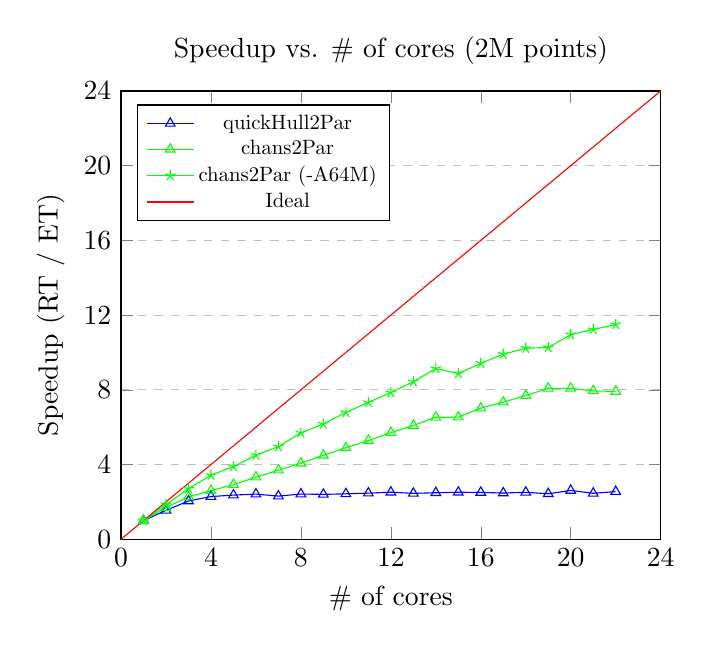
\begin{tikzpicture}
      \begin{axis}[
          title={Speedup vs. \# of cores (2M points)},
          xlabel={\# of cores},
          ylabel={Speedup (RT / ET)},
          xmin=0, xmax=24,
          ymin=0, ymax=24,
          xtick={0,4,8,12,16,20,24},
          ytick={0,4,8,12,16,20,24},
          legend style={nodes={scale=0.75, transform shape}},
          legend pos=north west,
          ymajorgrids=true,
          grid style=dashed,
      ]

      \addplot[
          color=blue,
          mark=triangle,
        ]
        coordinates {
        (1,1)(2,1.54766)(3,2.05005)(4,2.28538)(5,2.36471)(6,2.417191518)(7,2.309929296)(8,2.42067455)(9,2.402912687)(10,2.433525583)(11,2.46908561)(12,2.51971494)(13,2.457433727)(14,2.491329919)(15,2.516795146)(16,2.50704758)(17,2.475817205)(18,2.513555581)(19,2.436150603)(20,2.612431275)(21,2.460971795)(22,2.552342864)
        };
      \addplot[
          color=green,
          mark=triangle,
        ]
        coordinates {
        (1,1)(2,1.69786)(3,2.26924)(4,2.59934)(5,2.92666)(6,3.326271923)(7,3.698675957)(8,4.069636784)(9,4.496568747)(10,4.897876232)(11,5.290671544)(12,5.712284938)(13,6.090301589)(14,6.529305958)(15,6.53640421)(16,7.01912468)(17,7.341589225)(18,7.693612851)(19,8.07832577)(20,8.079111271)(21,7.94138577)(22,7.913967424)
        };
      \addplot[
          color=green,
          mark=star,
        ]
        coordinates {
        (1,1)(2,1.85533)(3,2.70513)(4,3.42966)(5,3.89266)(6,4.499545728)(7,4.96154334)(8,5.696202718)(9,6.170727018)(10,6.790000554)(11,7.325768293)(12,7.851378049)(13,8.436336996)(14,9.143209177)(15,8.868800463)(16,9.419725246)(17,9.9042208)(18,10.22569521)(19,10.2677308)(20,10.95362611)(21,11.22758824)(22,11.49630514)
        };
        
      \addplot[
          color=red,
          mark=none,
        ]
        coordinates {
        (0,0)(24,24)
        };
      \legend{quickHull2Par, chans2Par, chans2Par (-A64M), Ideal}
      \end{axis}
      \end{tikzpicture}
      \caption{A graph of speedup (calculated with $t_\text{Real} / t_\text{Elapsed}$) as a function of the \# of cores. We did not include quickHull3Par due it having almost identical performance to quickHull2. The star is just there to make it easier to differentiate between the two Chan's graphs; both are parallel.}
    \end{figure}

    The graph of speedup as a function of the number of cores tells us that Chan’s algorithm is much more parallelizable than QuickHull. This matches with what we expected, as the parallelizable portion of Chan’s takes up a much larger percentage of overall time when compared to the parallelizable portion of QuickHull.

    The plateau of each graph tells us roughly the maximum speedup of each algorithm. QuickHull plateaued at around 2.5x, Chan’s algorithm at around 8x, and Chan’s algorithm with an increased nursery size did not plateau whatsoever. Using Amdahl’s law, we can thus deduce that we parallelized roughly 60\% of the runtime of QuickHull, and roughly 87.5\% of the total runtime of Chan’s algorithm.

    Something we were not expecting was how effective increasing the size of the nursery would be for Chan’s algorithm. In fact, it was so effective that even up to 22 cores we were still observing a linear increase in speedup! This suggests that garbage collection takes up a large portion of the remaining non-parallelizable portion of Chan’s algorithm, which is a very good result.

    \begin{figure}[h!]
      \centering
      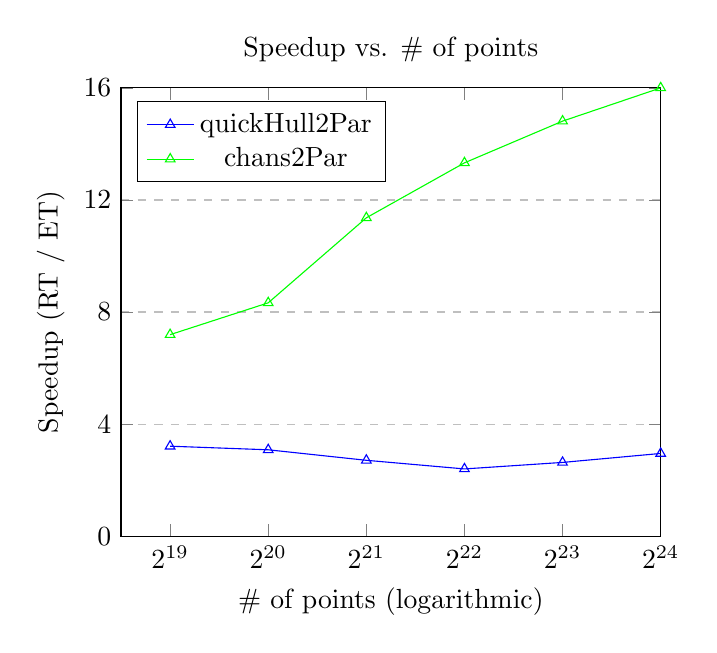
\begin{tikzpicture}
      \begin{axis}[
          title={Speedup vs. \# of points},
          xlabel={\# of points (logarithmic)},
          ylabel={Speedup (RT / ET)},
          log basis x = 2,
          xmode=log,
          xmax=16777216,
          ymin=0, ymax=16,
          xtick={524288,1048576,2097152,4194304,8388608,16777216},
          ytick={0,4,8,12,16},
          legend pos=north west,
          ymajorgrids=true,
          grid style=dashed,
      ]
      \addplot[
          color=blue,
          mark=triangle,
        ]
        coordinates {
          (524288,3.21196)(1048576,3.08365)(2097152,2.70869)(4194304,2.40076)(8388608,2.63301)(16777216,2.95295)
        };
      \addplot[
          color=green,
          mark=triangle,
        ]
        coordinates {
          (524288,7.19257)(1048576,8.32861)(2097152,11.3631)(4194304,13.32411)(8388608,14.81332)(16777216,15.99874)
        };
      \legend{quickHull2Par, chans2Par}
      \end{axis}
      \end{tikzpicture}
      \caption{A graph of speedup as a function of the \# of points.}
    \end{figure}
    
    For fun, we also decided to graph the speedup of the parallel functions as a function of the \# of points. Due to how $m$ was calculated, we suspected that larger values of $n$ may result in higher overall speedup, a theory proven correct with this graph.

    \newpage

    \begin{figure}[h]
      \centering
      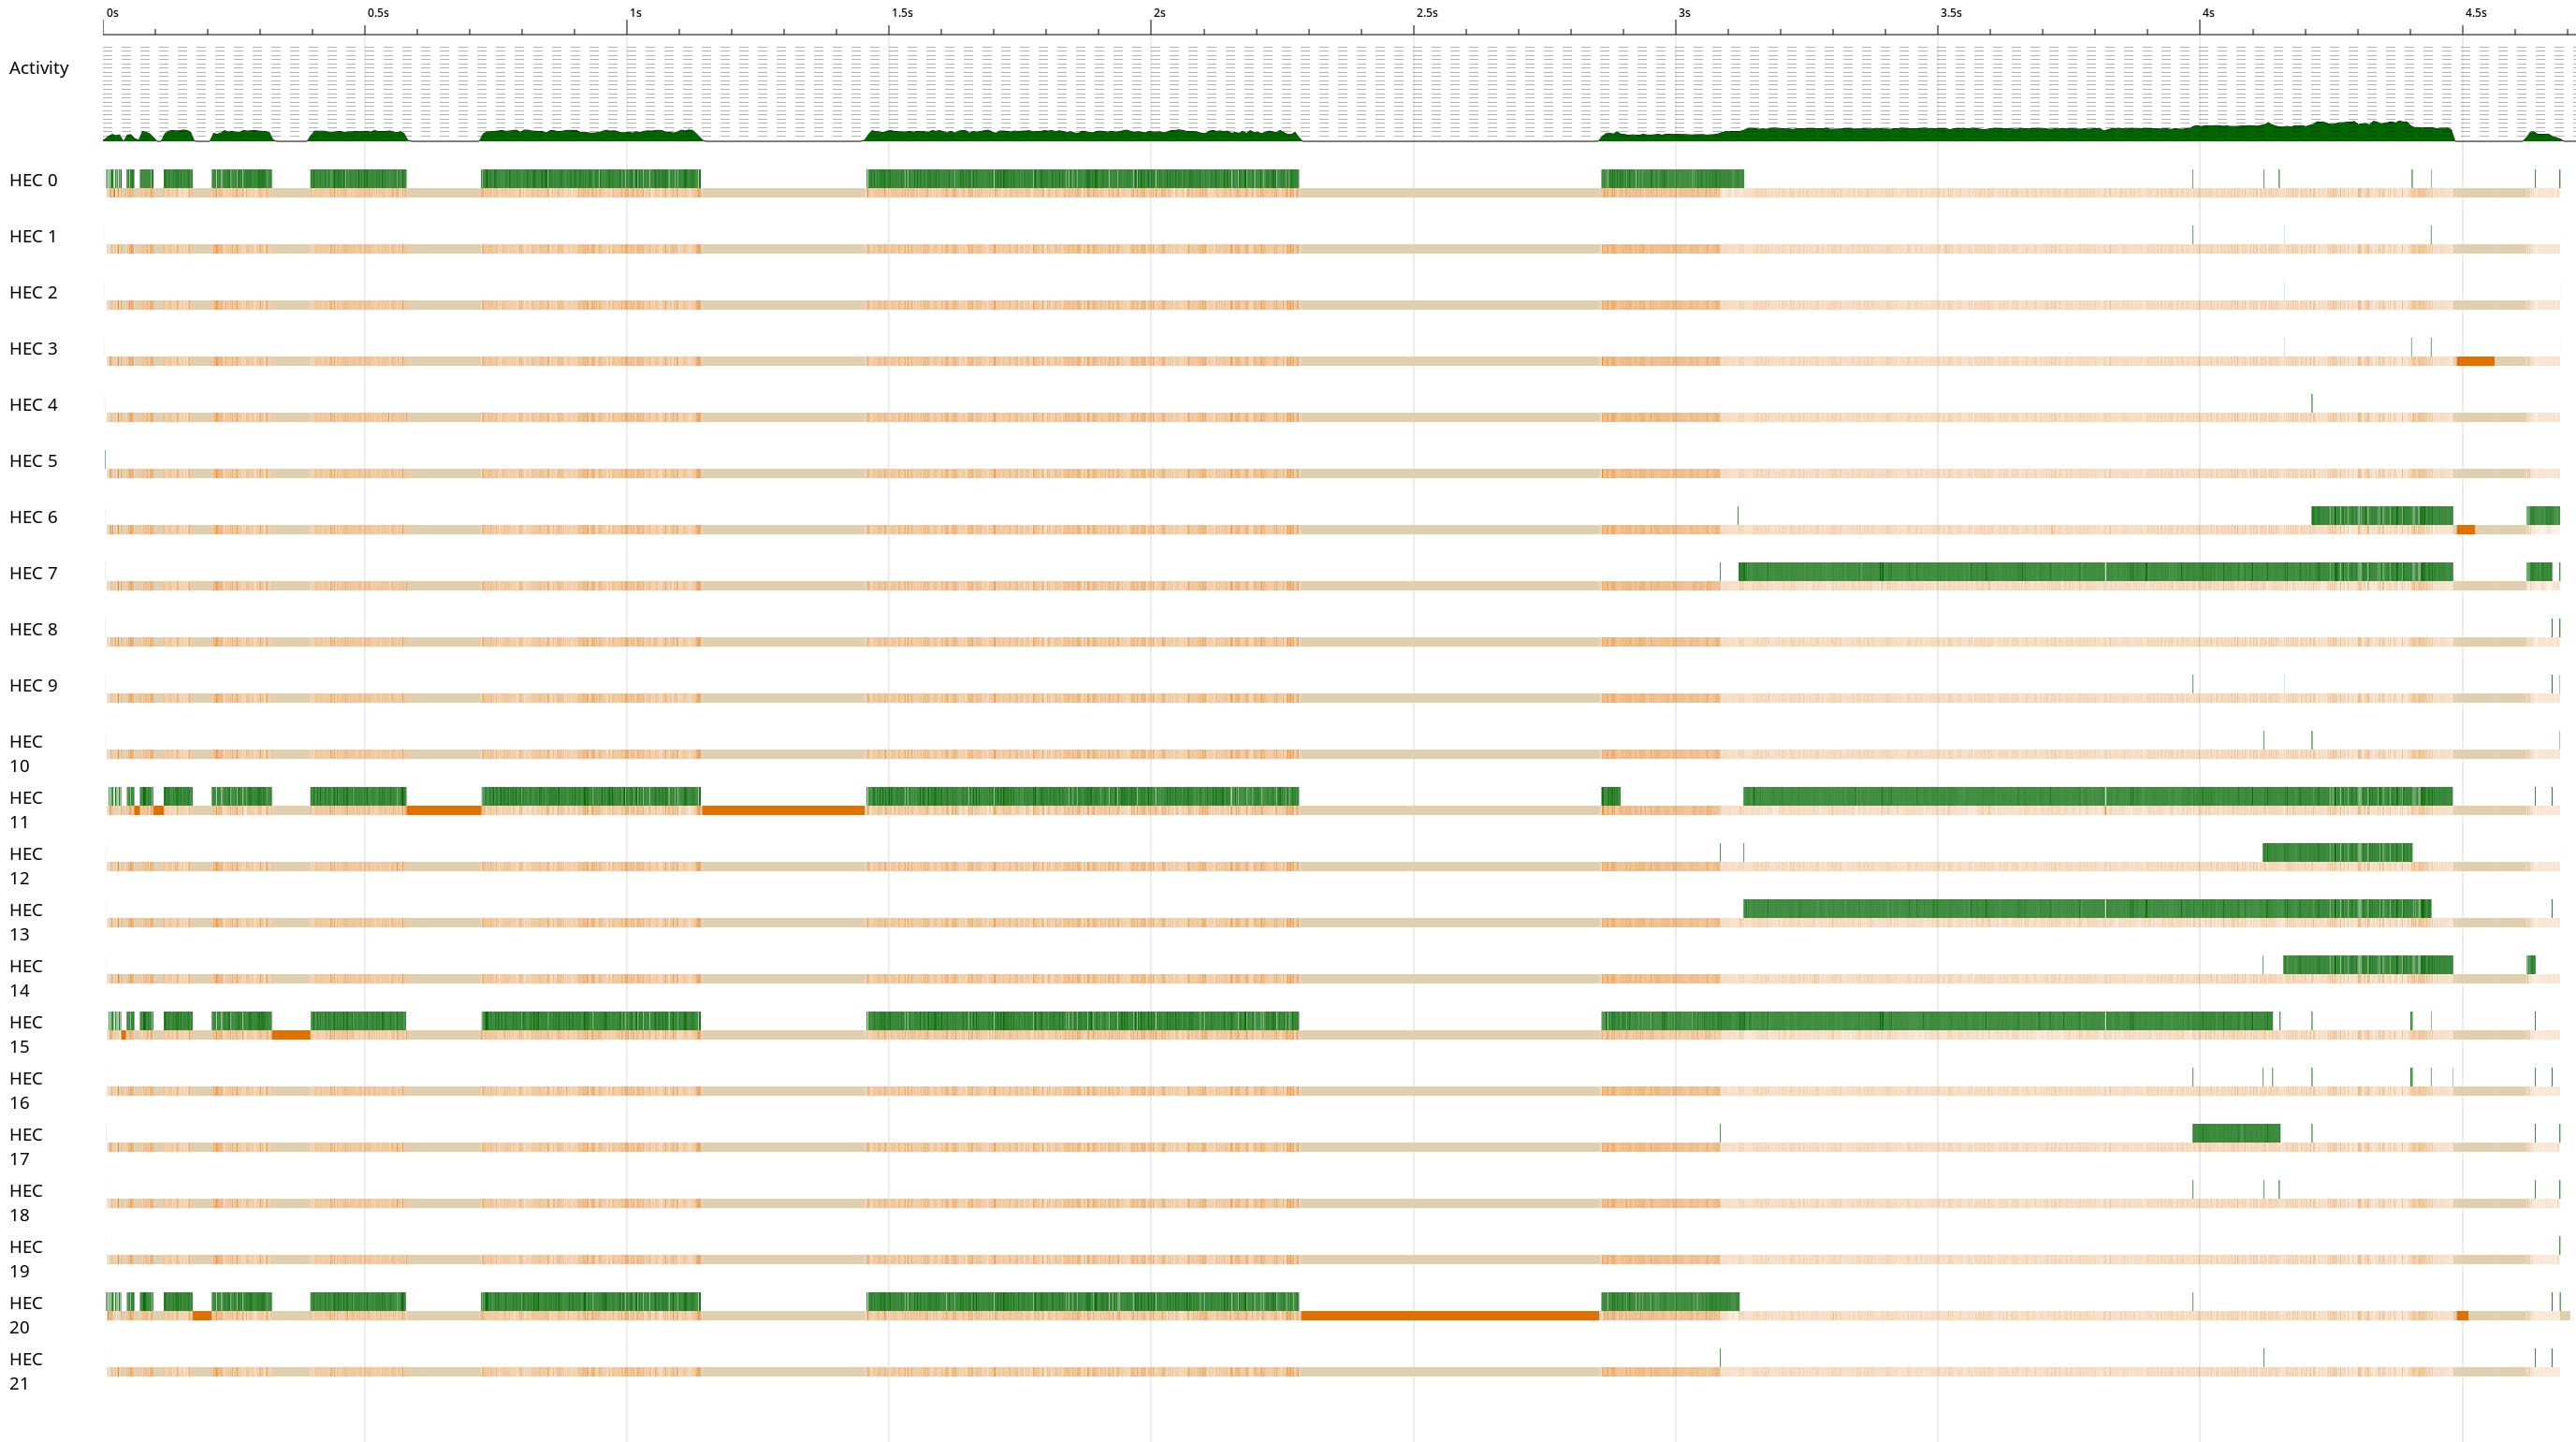
\includegraphics[width=0.75\textwidth]{quickhull2par_threadscope.png}
      \caption{A Threadscope log of QuickHull, with 22 threads and $2^{24}$ points.}
    \end{figure}

    The Threadscope log of QuickHull does not paint a pretty picture. For roughly two thirds of the time, only four threads are in use, and the remaining third does not show much parallel thread usage either. This result makes sense when considering that a very large number of points are discarded during the first partitioning of points, which when combined with the fact that each recursive sub-problem halves the number of points to process on average, means that sequential operations take up a large portion of the total runtime.

    \newpage

    \begin{figure}[h]
      \centering
      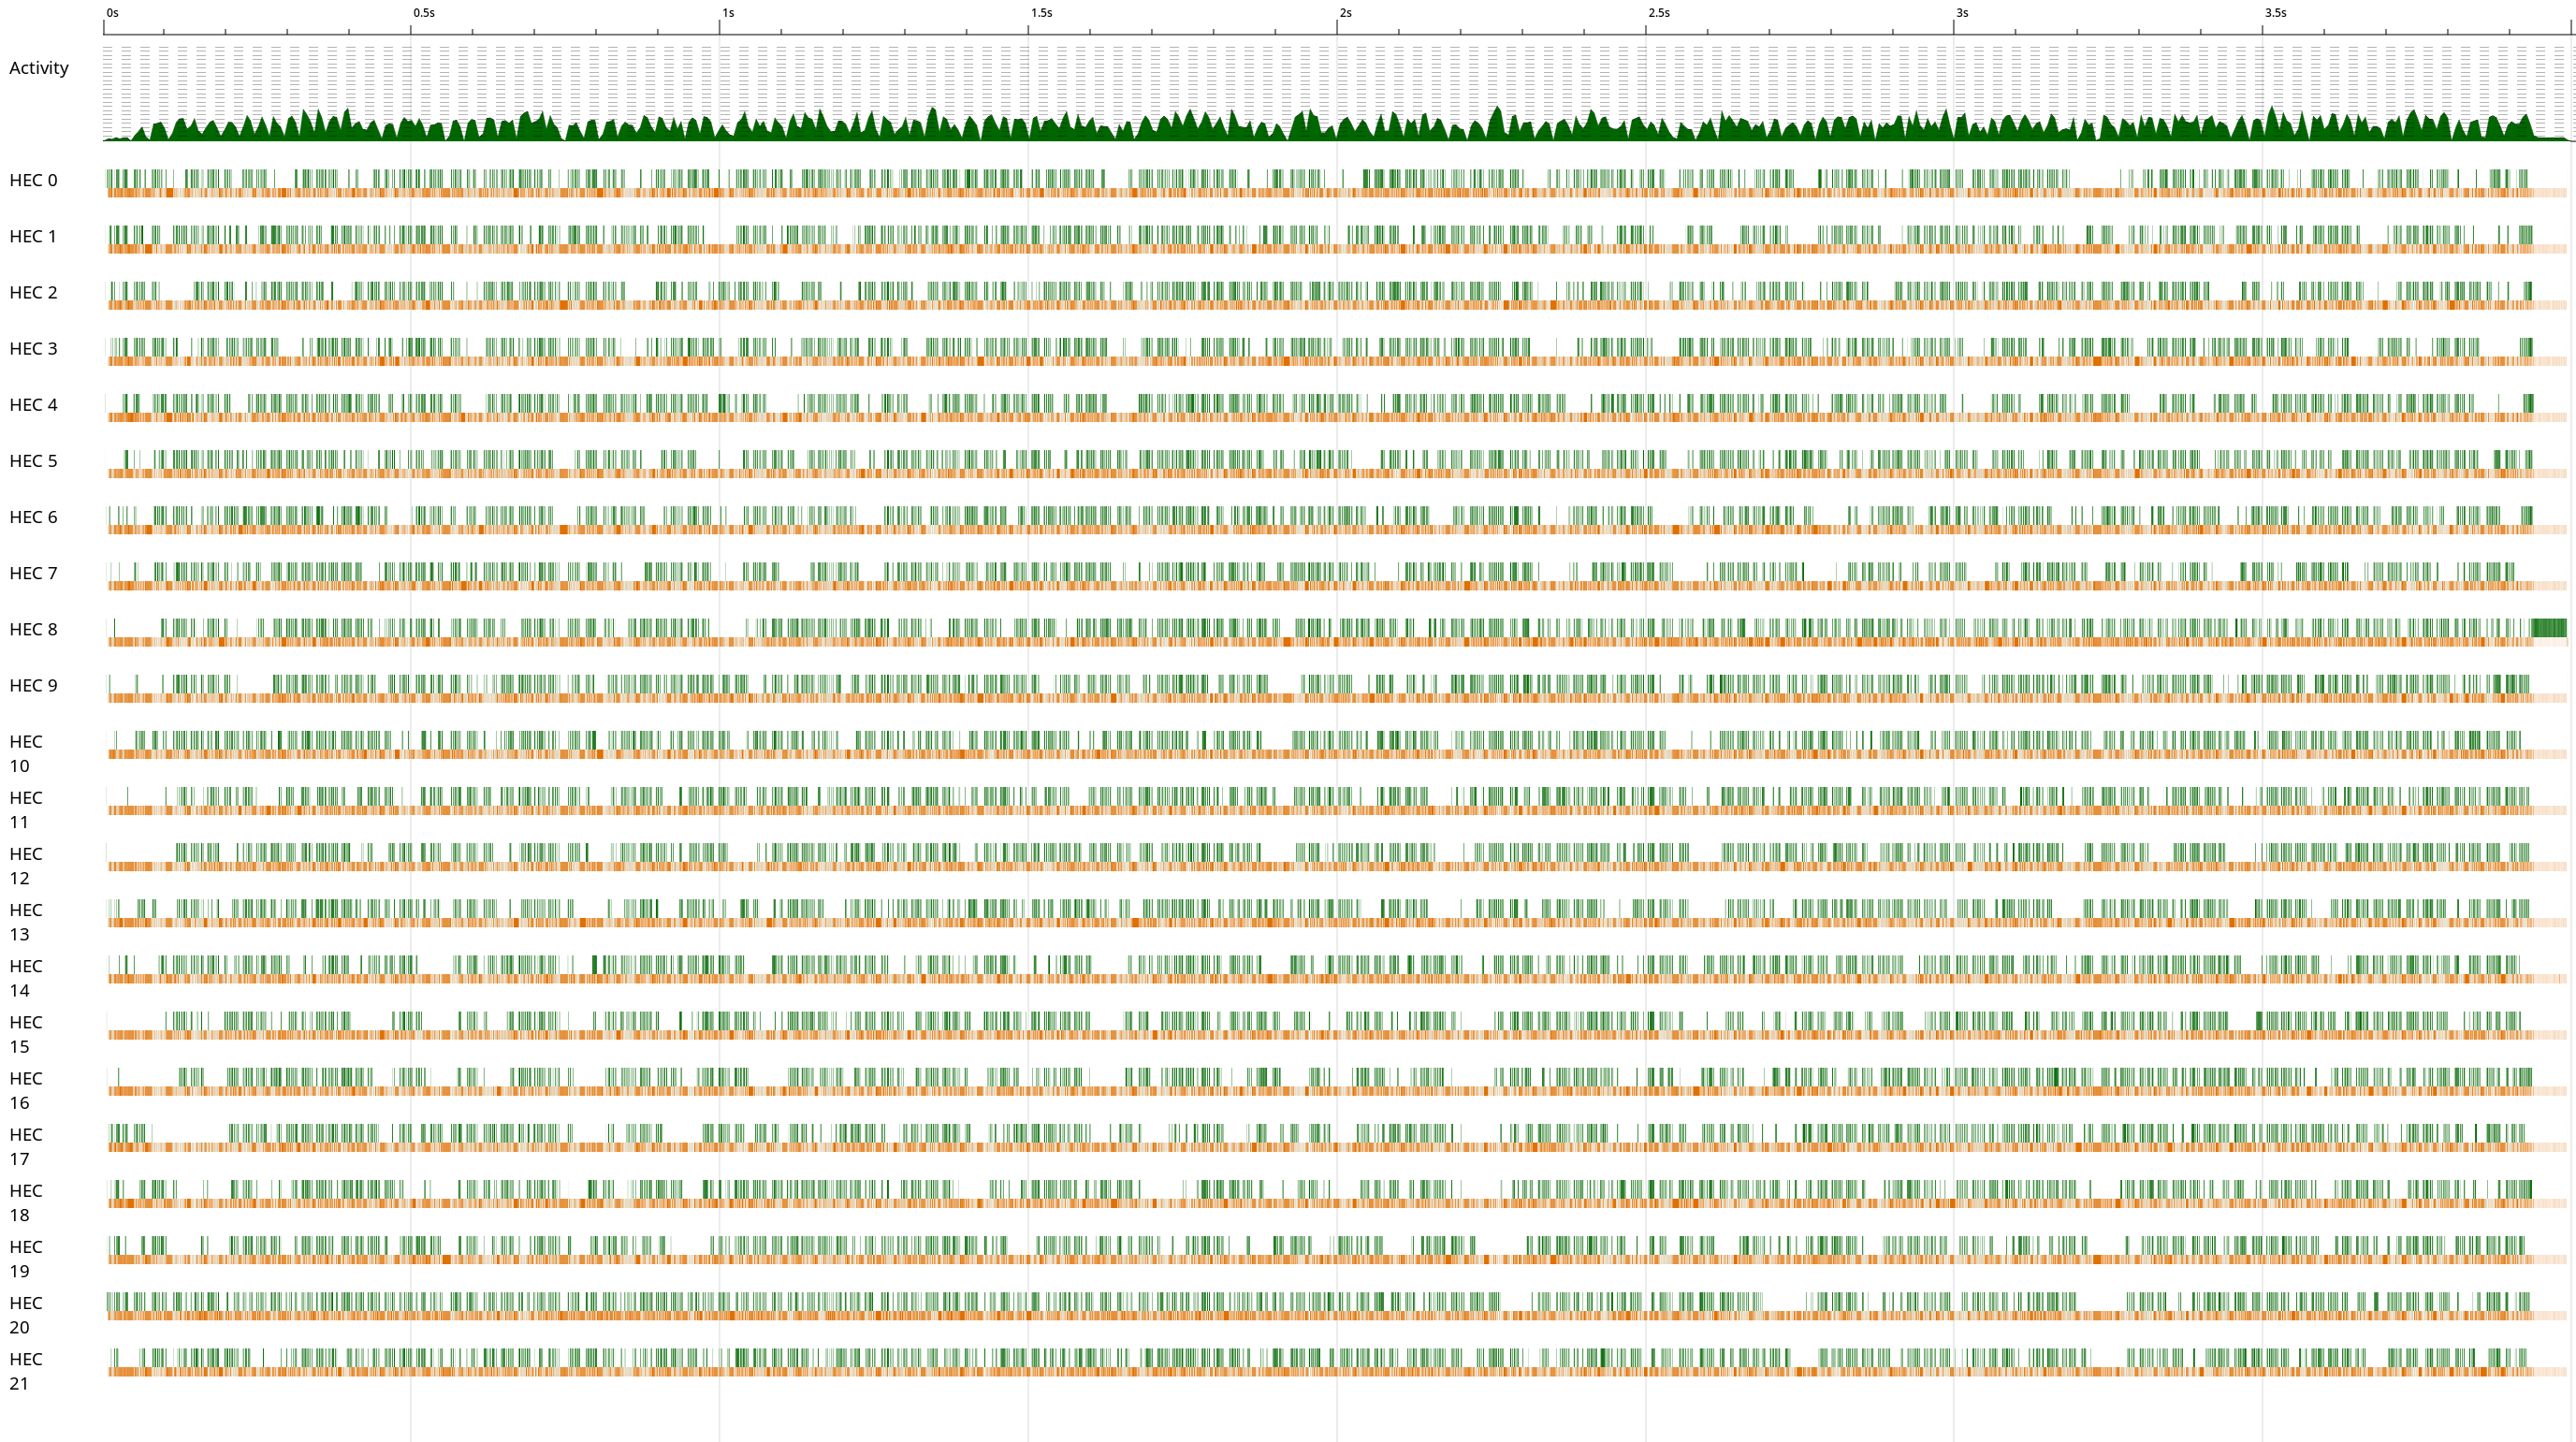
\includegraphics[width=0.75\textwidth]{chans2par_threadscope.png}
      \caption{A Threadscope log of Chan's algorithm, with 22 threads and $2^{24}$ points.}
    \end{figure}

    The threadscope log of Chan’s algorithm on the other hand showed much better results, as all threads have a roughly equal workload for the vast majority of the time. Furthermore, the log confirms our suspicion that the sequential portion of the algorithm (the joining of the sub-hulls) takes up a very small amount of the total runtime. However, the amount of garbage collection taking place along with the relatively low average activity is disappointing.

    \begin{figure}[h]
      \centering
      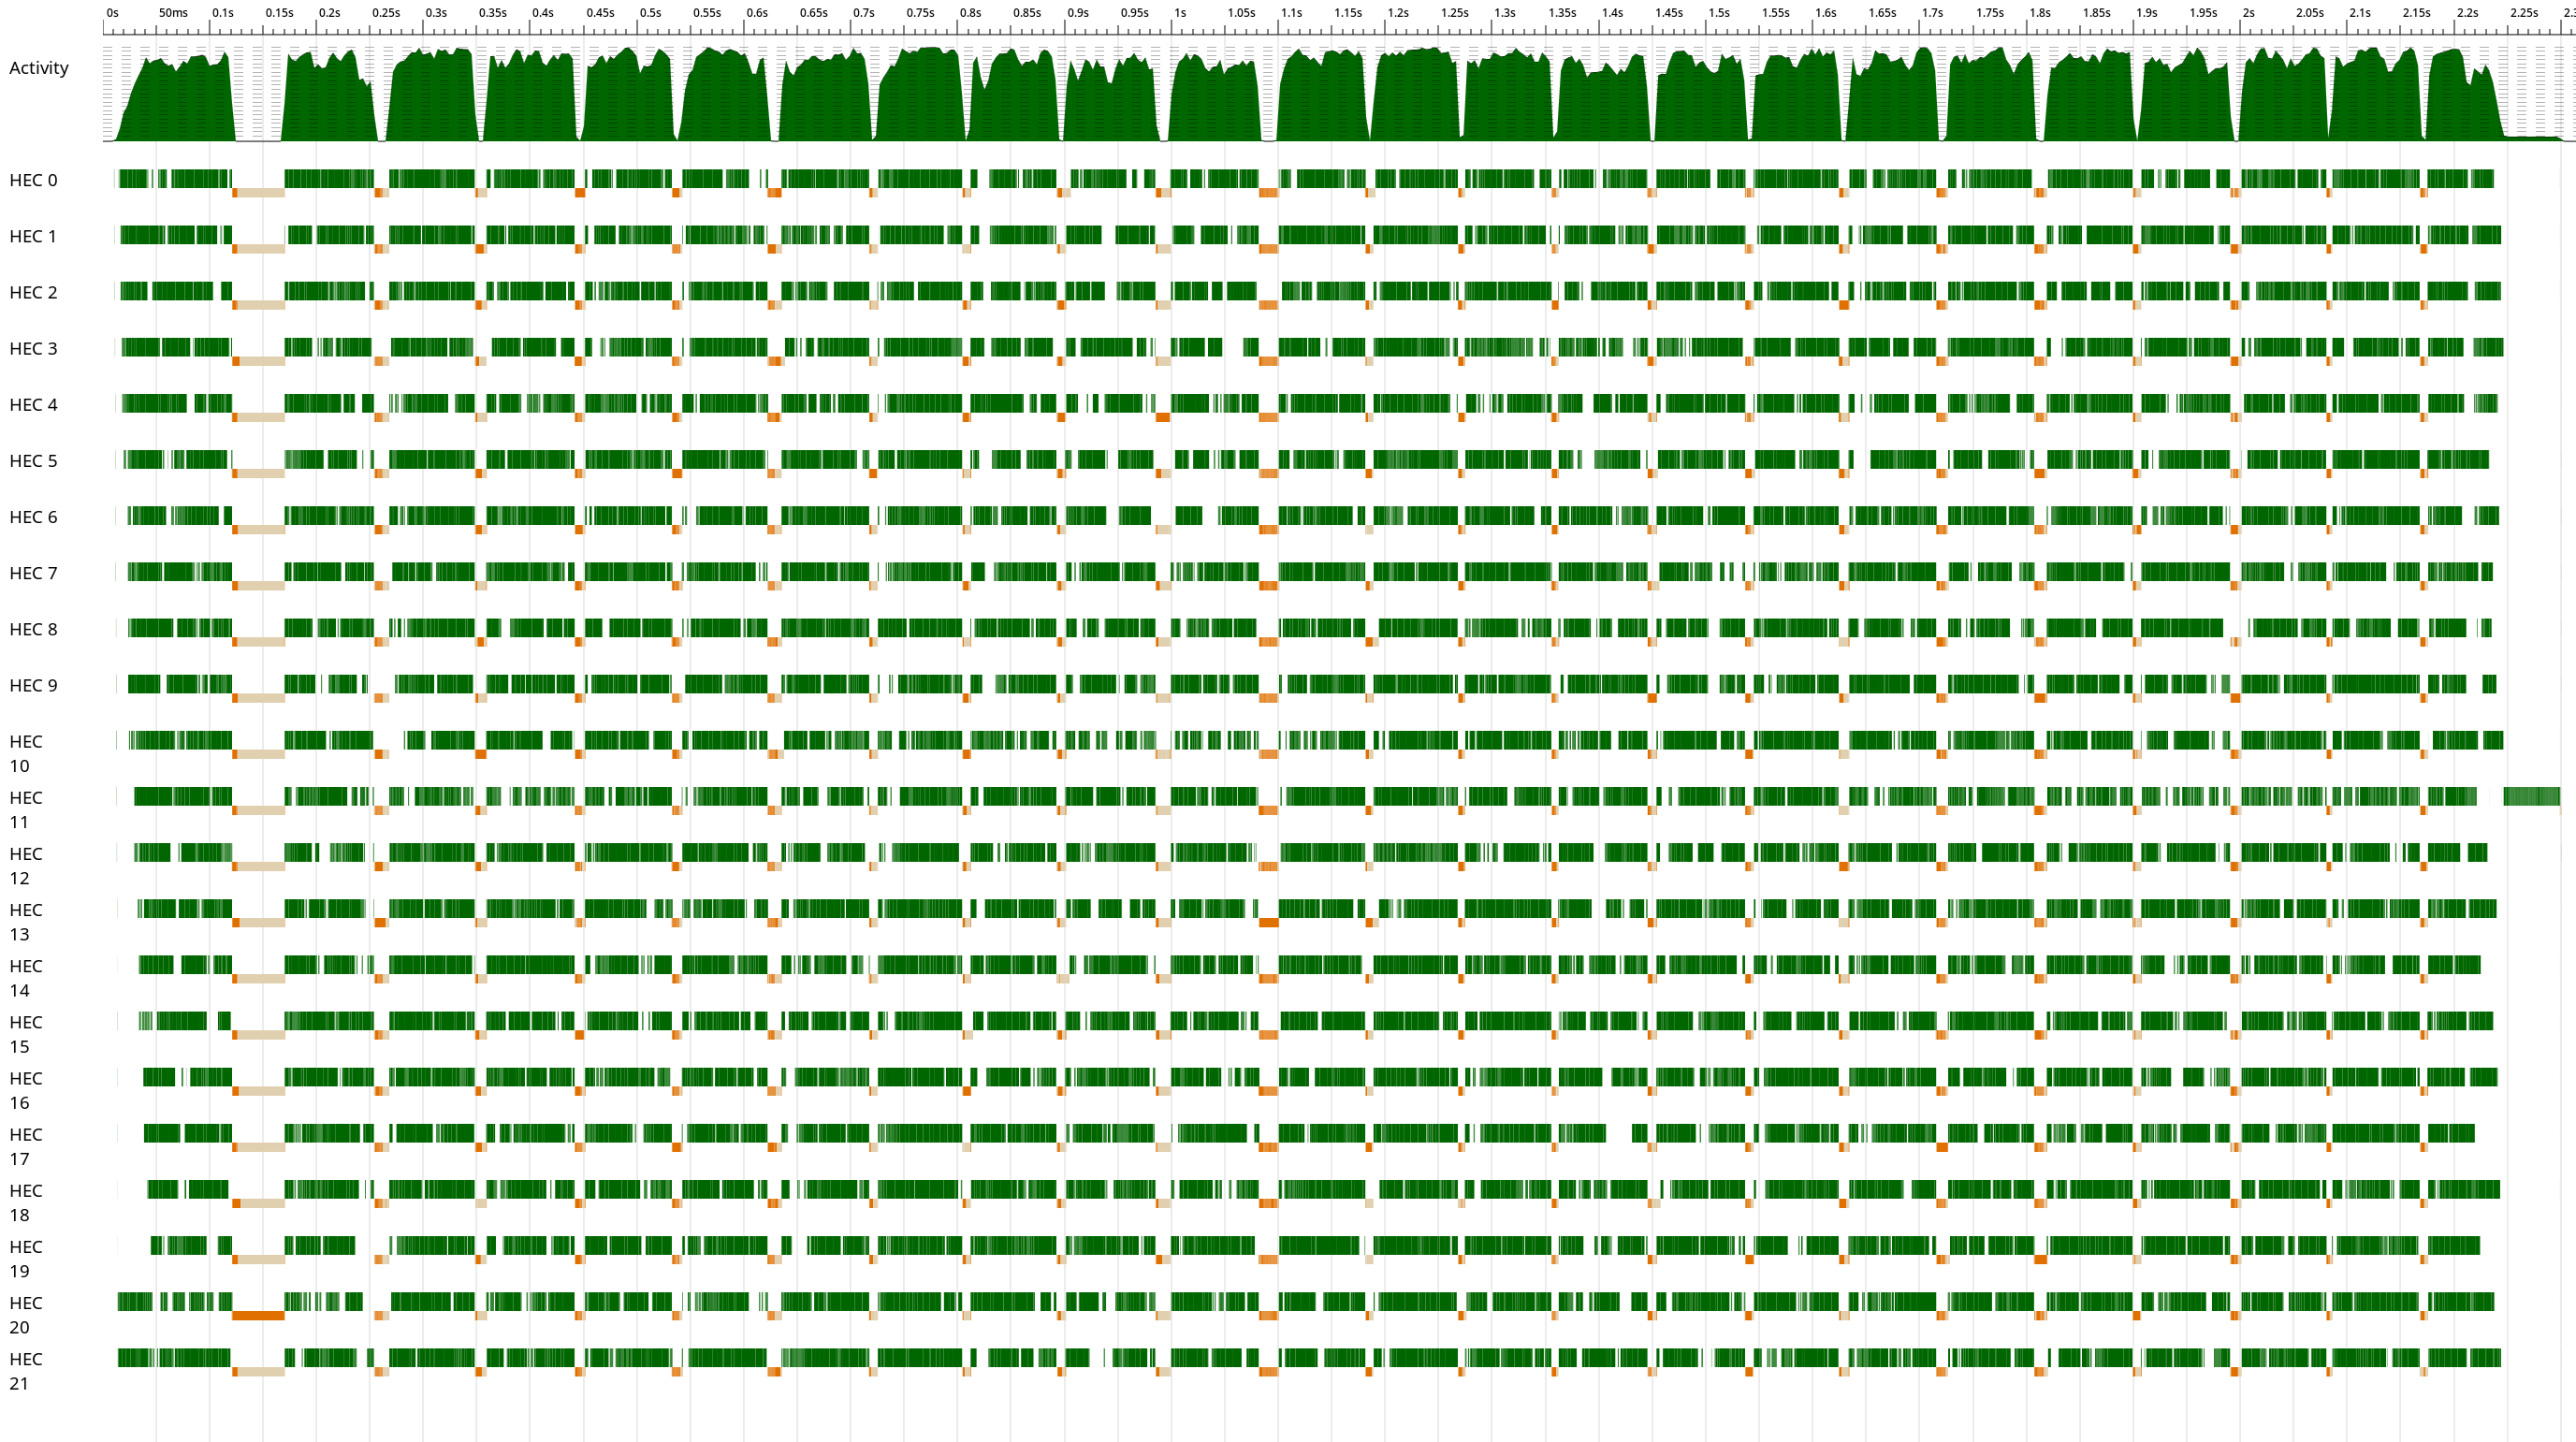
\includegraphics[width=0.75\textwidth]{chans2par_A64M_threadscope.png}
      \caption{A Threadscope log of Chan's algorithm, with 22 threads, $2^{24}$ points, and a 64MB nursery.}
    \end{figure}
    Luckily, the Threadscope log of Chan’s algorithm with an increased nursery size shows that increasing the nursery size eliminates both the problem of low activity and the problem of constant garbage collection. If it were not for the small sequential portion at the end, this Threadscope log shows that Chan’s algorithm with an increased nursery size is an almost perfectly parallelizable algorithm!

  \newpage
  \section*{Code}

    \subsection*{Shared (Lib.hs)}

    \begin{minted}[fontsize=\small, linenos]{haskell}
isCCWTurn :: (Ord a, Num a) => V2 a -> V2 a -> V2 a -> Bool
isCCWTurn o p1 p2 = crossZ (p1 - o) (p2 - o) >= 0

squareDistance2 :: (Num a) => V2 a -> V2 a -> a
squareDistance2 (V2 x0 y0) (V2 x1 y1) = dx * dx + dy * dy
 where
  dx = x1 - x0
  dy = y1 - y0

-- Calculate distance from line
distFromLine2 :: (Num a) => V2 a -> V2 a -> V2 a -> a
distFromLine2 p0 p1 = crossZ (p1 - p0) . subtract p0

-- GT = o -> p1 -> p2 is a counter-clockwise turn
-- LT = o -> p1 -> p2 is a clockwise turn
-- EQ = o, p1, and p2 are colinear, instead compare based on distance
orientation :: (Ord a, Num a) => V2 a -> V2 a -> V2 a -> Ordering
orientation p0 p1 p2 = compare (crossZ (p1 - p0) (p2 - p0)) 0 \
  <> compare (squareDistance2 p0 p1) (squareDistance2 p0 p2)

-- Sort a list of points in counter-clockwise order starting from the point
-- with the lowest x value
sortPointsCW :: (Ord a, Num a) => [V2 a] -> [V2 a]
sortPointsCW [] = []
sortPointsCW points =
  let o = minimum points -- o is the minimum with respect to x, then to y
   in o : (sortBy (orientation o) . filter (/= o)) points

-- Sort a list of points in counter-clockwise order starting from the point
-- with the lowest x value
sortPointsCCW :: (Ord a, Num a) => [V2 a] -> [V2 a]
sortPointsCCW [] = []
sortPointsCCW points =
  let o = minimum points -- o is the minimum with respect to x, then to y
   in o : (sortBy (flip (orientation o)) . filter (/= o)) points
  \end{minted}

  \subsection*{Graham Scan}

  \begin{minted}[fontsize=\small, linenos]{haskell}
angleToXAxis :: (RealFloat a) => V2 a -> V2 a -> a
angleToXAxis (V2 x0 y0) (V2 x y) = atan2 (y - y0) (x - x0)

sortPointsByAngle :: (RealFloat a) => V2 a -> ([V2 a] -> [V2 a])
sortPointsByAngle p0 = sortOn (angleToXAxis p0)

buildHull :: (RealFloat a) => [V2 a] -> [V2 a] -> [V2 a]
buildHull hull [] = hull -- base case: no more points
buildHull (p1 : p0 : hull) (p : points)
  -- left turn or collinear: add p to the hull and continue
  | isCCWTurn p0 p1 p = buildHull (p : p1 : p0 : hull) points
  -- right turn: pop p1 from hull and continue
  | otherwise = buildHull (p0 : hull) (p : points)
  -- if there are less than 2 points, just push p onto hull and continue
buildHull hull (p : points) = buildHull (p : hull) points

grahamScan :: (RealFloat a) => [V2 a] -> [V2 a]
grahamScan [] = []
grahamScan p@[_] = p
grahamScan p@[_, _] = p
grahamScan p@[_, _, _] = p
grahamScan points =
  let pYMin = minimumBy (\(V2 _ ay) (V2 _ by) -> compare ay by) points
      sortedPoints = sortPointsByAngle pYMin points
      convexHull = buildHull [] sortedPoints
   in convexHull
  \end{minted}

  \subsection*{QuickHull}

    \begin{minted}[fontsize=\small, linenos]{haskell}
quickHull2 :: (Ord a, Num a) => [V2 a] -> [V2 a]
quickHull2 points =
  let
    _quickHull2 :: (Num a, Ord a) => [V2 a] -> V2 a -> V2 a -> [V2 a]
    _quickHull2 ps p0 p1
      | null ps = [p1]
      | otherwise =  _quickHull2 onRight pm p1 ++ _quickHull2 onLeft p0 pm
     where
      pm = maximumBy (compare `on` distFromLine2 p0 p1) ps
      (onLeft, maybeOnRight) = partition ((> 0) . distFromLine2 p0 pm) ps
      onRight = filter ((> 0) . distFromLine2 pm p1) maybeOnRight

    pXMin = minimumBy (compare `on` (^. _x)) points
    pXMax = maximumBy (compare `on` (^. _x)) points

    (topPoints, bottomPoints) = partition ((> 0) . distFromLine2 pXMin pXMax) points

  in if (null . drop 3) points then points else _quickHull2 topPoints pXMin pXMax \
    ++ _quickHull2 bottomPoints pXMax pXMin

quickHull2Par :: (Num a, Ord a, NFData a) => [V2 a] -> [V2 a]
quickHull2Par points =
  let maxDepth = 100
      _quickHull2Par :: (Num a, Ord a, NFData a) => Int -> [V2 a] -> (V2 a, V2 a) -> [V2 a]
      _quickHull2Par d ps (p0, p1)
        | null onLeft = [p0]
        | d < maxDepth = concat (map (_quickHull2Par (d + 1) onLeft) nextLines \
            `using` parList rdeepseq)
        | otherwise = concatMap (_quickHull2Par (d + 1) onLeft) nextLines
       where
        onLeftDists = (filter ((> 0) . snd) . map (\p -> (p, distFromLine2 p0 p1 p))) ps
        onLeft = map fst onLeftDists
        pm = (fst . maximumBy (compare `on` snd)) onLeftDists
        nextLines = [(p0, pm), (pm, p1)]

      maxXPoint = maximumBy (compare `on` (^. _x)) points
      minXPoint = minimumBy (compare `on` (^. _x)) points
      maxYPoint = maximumBy (compare `on` (^. _y)) points
      minYPoint = minimumBy (compare `on` (^. _y)) points
      --
      topLeft = (minXPoint, maxYPoint)
      topRight = (maxYPoint, maxXPoint)
      bottomRight = (maxXPoint, minYPoint)
      bottomLeft = (minYPoint, minXPoint)

   in if (null . drop 3) points then points else concat (map (_quickHull2Par 1 points) \
    [topLeft, topRight, bottomRight, bottomLeft] `using` parList rdeepseq)
    \end{minted}

    \begin{minted}[fontsize=\footnotesize, linenos]{haskell}
-- Face representation as described in Section 1: "We represent a convex hull
-- with a set of facets and a set of adjacency lists"
data Face a = Face {vertices :: (V3 a, V3 a, V3 a), \
  outsideSet :: [(V3 a, a)], furthestPoint :: Maybe (V3 a, a)}

-- Based on geometric orientation test described in Section 2: Signed volume
-- calculation for determining if point is above face
signedVolume :: Floating a => V3 a -> V3 a -> V3 a -> V3 a -> a
signedVolume a b c = dot (cross (b - a) (c - a)) . subtract a

-- Find points above a plane with distance
findPointsAbove :: (Ord a, Floating a) => a -> V3 a -> V3 a -> V3 a -> [V3 a] -> [(V3 a, a)]
findPointsAbove epsilon p0 p1 p2 points = let volumes = [(p, vol) | p <- points, \
  p /= p0 && p /= p1 && p /= p2, let vol = signedVolume p0 p1 p2 p, vol > epsilon] \
  in volumes

-- Create initial faces of tetrahedron
createInitialFaces :: (Ord a, Floating a) => a -> [V3 a] -> V3 a -> V3 a -> V3 a -> V3 a -> [Face a]
createInitialFaces epsilon points p0 p1 p2 p3 = 
    let faces = [(p0, p1, p2), (p0, p2, p3), (p0, p3, p1), (p1, p3, p2)]
        remainingPoints = filter (\p -> p /= p0 && p /= p1 && p/= p2 && p /= p3) points
        createFace (v1, v2, v3) = 
            let outside = findPointsAbove epsilon v1 v2 v3 remainingPoints
                furthest = if null outside then Nothing else Just $ maximumBy \
                  (compare `on` snd) outside
            in Face (v1, v2, v3) outside furthest
    in map createFace faces

-- Process a face using Beneath-Beyond method
processFace :: (Ord a, Floating a) => a -> Face a -> [(V3 a, V3 a, V3 a)]
processFace epsilon face =
    case furthestPoint face of
        Nothing -> [vertices face]
        Just (p, _) -> 
            let (v1, v2, v3) = vertices face
                -- Create cone of new faces (Section 1)
                newFaces = [(v1, v2, p), (v2, v3, p), (v3, v1, p)]
                remainingPoints = map fst $ filter ((/= p) . fst) $ outsideSet face
                processNewFace (a, b, c) = 
                    let outside = findPointsAbove epsilon a b c remainingPoints
                    in if null outside
                       then [(a, b, c)]
                       else let furthest = maximumBy (compare `on` snd) outside
                            in processNewFaceWithPoints epsilon outside furthest (a, b, c)
            in concatMap processNewFace newFaces


-- Process new faces recursively with their outside sets
processNewFaceWithPoints :: (Ord a, Floating a) => a -> [(V3 a, a)] -> (V3 a, a) \
  -> (V3 a, V3 a, V3 a) -> [(V3 a, V3 a, V3 a)]
processNewFaceWithPoints epsilon points furthest (a, b, c) =
    let (fp, _) = furthest
        remaining = map fst $ filter ((/= fp) . fst) points
    in if null remaining
       then [(a, b, c)]
       else let newFaces = [(a, b, fp), (b, c, fp), (c, a, fp)]
                processSubFace (v1, v2, v3) =
                    let above = findPointsAbove epsilon v1 v2 v3 remaining
                    in if null above
                       then [(v1, v2, v3)]
                       else let (p', _) = maximumBy (compare `on` snd) above
                            in processNewFaceWithPoints epsilon above \
                              (p', snd furthest) (v1, v2, v3)
            in concatMap processSubFace newFaces

-- Sequential
quickHull3 :: (Ord a, Floating a) => [V3 a] -> [V3 a]
quickHull3 points 
    | length points < 4 = points
    | otherwise = 
        let epsilon = 1e-8 -- Numerical tolerance from Section 4
            -- Initial point selection as described in Section 2
            p0 = minimumBy (compare `on` (^._x)) points
            p1 = maximumBy (compare `on` distance p0) points
            rest1 = filter (\p -> p /= p0 && p /= p1) points
            p2 = maximumBy (compare `on` \p -> norm (cross (p1 - p0) (p - p0))) rest1
            rest2 = filter (/= p2) rest1
            p3 = maximumBy (compare `on` \p -> abs $ signedVolume p0 p1 p2 p) rest2
            initialFaces = createInitialFaces epsilon points p0 p1 p2 p3
            allTriangles = concatMap (processFace epsilon) initialFaces
        in nub $ concatMap (\(a,b,c) -> [a,b,c]) allTriangles

-- Parallel face processing based on Section 3's discussion of algorithm variations
processPointsParallel :: (Ord a, Floating a, NFData a) => Int -> a -> [V3 a] -> \
  Face a -> [(V3 a, V3 a, V3 a)]
processPointsParallel depth epsilon points face =
    case furthestPoint face of
        Nothing -> [vertices face]
        Just (p, _) -> 
            let (v1, v2, v3) = vertices face
                newFaces = [(v1, v2, p), (v2, v3, p), (v3, v1, p)]
                remainingPoints = map fst $ filter ((/= p) . fst) $ outsideSet face
                processNewFace (a, b, c) = 
                    let outside = findPointsAbove epsilon a b c remainingPoints
                        newFace = Face (a,b,c) outside (if null outside 
                                                      then Nothing 
                                                      else Just $ maximumBy \
                                                        (compare `on` snd) outside)
                    in if depth < 64
                       then processPointsParallel (depth + 1) epsilon points newFace
                       else processFace epsilon newFace
            in if depth < 2
               then concat (map processNewFace newFaces `using` parList rdeepseq)
               else concatMap processNewFace newFaces

-- Parallel
quickHull3Par :: (Ord a, Floating a, NFData a) => [V3 a] -> [V3 a]
quickHull3Par points 
    | length points < 4 = points
    | otherwise = 
        let epsilon = 1e-8
            p0 = minimumBy (compare `on` (^._x)) points
            p1 = maximumBy (compare `on` distance p0) points
            rest1 = filter (\p -> p /= p0 && p /= p1) points
            p2 = maximumBy (compare `on` \p -> norm (cross (p1 - p0) (p - p0))) rest1
            rest2 = filter (/= p2) rest1
            p3 = maximumBy (compare `on` \p -> abs $ signedVolume p0 p1 p2 p) rest2
            initialFaces = createInitialFaces epsilon points p0 p1 p2 p3
            allTriangles = concat (map (processPointsParallel 0 epsilon points) \
              initialFaces `using` parList rdeepseq)
        in nub $ concatMap (\(a,b,c) -> [a,b,c]) allTriangles
    \end{minted}

  \subsection*{Chan's}

    \begin{minted}[fontsize=\small, linenos]{haskell}
chansJarvisMarch :: (Num a, Ord a) => [V.Vector (V2 a)] -> V2 a -> V2 a -> [V2 a]
chansJarvisMarch subHulls start p =
  let next = maximumBy (orientation p) $ map (rightmostPoint p) subHulls
    in if next == start then [p] else p : chansJarvisMarch subHulls start next

rightmostPoint :: (Ord a, Num a) => V2 a -> V.Vector (V2 a) -> V2 a
rightmostPoint o ps = ps V.! binarySearch 0 (V.length ps - 1) lPrevInit lNextInit
 where
  compareAdjacent i = (prev, next)
   where
    prev = orientation o (ps V.! i) (ps V.! ((i - 1) `mod` V.length ps))
    next = orientation o (ps V.! i) (ps V.! ((i + 1) `mod` V.length ps))

  -- We can save some computations here if we pass the orientations of the
  -- leftmost node, since those only need to be recalculated when l changes
  (lPrevInit, lNextInit) = compareAdjacent 0

  binarySearch l r lPrevOri lNextOri
    -- If we can't reach anymore points, we'll do l
    | l >= r = l
    -- If o->m->m-1 is not a CCW turn, and o->m->m+1 is not CCW turn, we are at
    -- the rightmost point!
    | mPrevOri /= LT && mNextOri /= LT = m
    -- If o->l->m is a CCW turn and (o->l->l+1 is a CW turn or o->l->l-1 and
    -- o->l->l+1 turn the same way), or o->l->m is a CW turn and o->m->m-1 is a
    -- CW turn, then search to the right of m (from l to m)
    | mLOri == GT && (lNextOri == LT || lPrevOri == lNextOri) \
      || mLOri == LT && mPrevOri == LT = binarySearch l m lPrevOri lNextOri
    -- Otherwise, search to the left of m (from m+1 to r) (new lPrev = -mNext,
    -- new lNext needs to be set manually)
    | otherwise = binarySearch (m + 1) r (compare EQ mNextOri) \ 
      (orientation o (ps V.! (m + 1)) (ps V.! ((m + 2) `mod` V.length ps)))
   where
    m = (l + r) `div` 2
    -- Which side is m on, relative to l?
    mLOri = orientation o (ps V.! l) (ps V.! m) 
    -- What are the orientations of o->m->m-1 and o->m->m+1?
    (mPrevOri, mNextOri) = compareAdjacent m 

chans2 :: (Ord a, Num a) => Int -> [V2 a] -> [V2 a]
chans2 n ps = chansJarvisMarch subHulls start start
 where
  -- 3 * sqrt(A) is a good approximation of the perimeter of a polygon with
  -- area A
  m = 3 * (floor . sqrtDouble . fromIntegral) n 
  subPoints = chunksOf m ps
  -- V.force lets us save on space (forces vector capacity == vector length)
  subHulls = map (V.force . V.fromList . quickHull2) subPoints
  start = minimumBy (compare `on` (^. _x)) $ map (V.minimumOn (^. _x)) subHulls

chans2Par :: (Ord a, Num a, NFData a) => Int -> [V2 a] -> [V2 a]
chans2Par n ps = chansJarvisMarch subHulls start start
 where
  m = 3 * (floor . sqrtDouble . fromIntegral) n
  subPoints = chunksOf m ps
  subHulls = map (V.force . V.fromList . quickHull2) subPoints \
    `using` parBuffer 32 rdeepseq -- Here's the parallelization
  start = minimumBy (compare `on` (^. _x)) $ map (V.minimumOn (^. _x)) subHulls
    \end{minted}

  \newpage
  \printbibliography

\end{document}
